\pagebreak
\nolinenumbers
\section{Example: breadth first search with GraphBLAS}
{\scriptsize
\lstinputlisting[language=C,numbers=left]{BFS5M.c}
}

\pagebreak
\nolinenumbers
\section{Example: betweenness centrality with GraphBLAS}
{\scriptsize
\lstinputlisting[language=C,numbers=left]{BC1M.c}
}

\comment{
\pagebreak
\linenumbers
\section{Algebraless option}

\subsection{Vector-matrix multiply ({\sf vxm})}

Multiplies a vector by a matrix. The result is a vector.

\paragraph{C99 Syntax}

\begin{verbatim}
#include "GraphBLAS.h"
GrB_info GrB_vxm(GrB_Vector *u, const GrB_operation f, const GrB_operation g,
         const GrB_Vector v, const GrB_Matrix A
         [, const GrB_Vector m[, const GrB_Descriptor d]])
\end{verbatim}

\paragraph{Input Parameters}

\begin{itemize}
	\item[{\sf f}] ({\sf ARG0}) Additive operation used in the vector-matrix
	multiply.

	\item[{\sf g}] ({\sf ARG1}) Multiplicative oepration useind in the vector-matrix multiply.

	\item[{\sf v}] ({\sf ARG2}) Vector to be multiplied.

	\item[{\sf A}] ({\sf ARG3}) Matrix to be multiplied.

	\item[{\sf m}] ({\sf MASK}) Operation mask (optional). The mask
	specifies which elements of the result vector are to be computed.
	If no mask is necessary (i.e., compute all elements of result
	vector), {\sf GrB\_NULL} can be used or the mask can be omitted.

	\item[{\sf d}] Operation descriptor (optional). The descriptor
	is used to specify details of the operation, such as transpose
	the matrix or not, invert the mask or not (see below). If a
	\emph{default} descriptor is desired, {\sf GrB\_NULL} can be
	used or the descriptor can be omitted.
\end{itemize}

\paragraph{Output Parameter}

\begin{itemize}
	\item[{\sf u}] ({\sf OUTP}) Address of result vector.
\end{itemize}

\paragraph{Return Value}

\begin{tabular}{rl} 
{\sf GrB\_SUCCESS} 	& operation completed successfully \\
{\sf GrB\_PANIC}	& unknown internal error \\
{\sf GrB\_OUTOFMEM}	& not enough memory available for operation \\
{\sf GrB\_MISMATCH}	& mismatch among vectors, matrix and/or algebra
\end{tabular}

\paragraph{Description}

Let $\otimes: D_1 \times D_2 \rightarrow D_3$ and $\oplus: D_3 \times
D_3 \rightarrow D_3$ be the operations defined by arguments {\sf f}
and {\sf g}, respectively.

Vectors $\vector{v}, \vector{m}$ and matrix $\matrix{A}$ are computed
from input parameters {\sf v}, {\sf m} and {\sf A}, respectively,
as specified by descriptor {\sf d}.  $\bold{D}(\vector{v}) = D_1$ and
$\bold{D}(\matrix{A}) = D_2$.  $\bold{D}(\vector{m}) = {\sf GrB\_BOOL}$.
If {\sf m} is {\sf GrB\_NULL} then $\vector{m}$ is a Boolean vector of
size $\bold{n}(\vector{A})$ and with all elements set to {\sf true}.

If either $\vector{v}, \vector{m}$ or $\matrix{A}$ cannot be computed
from the input parameters as described above, the method returns {\sf
GrB\_MISMATCH}.

A consistency check is performed to verify that $\bold{n}(\vector{v})
= \bold{m}(\matrix{A})$ and $\bold{n}(\vector{m}) =
\bold{n}(\matrix{A})$. If a consistency check fails, the operation is
aborted and the method returns {\sf GrB\_MISMATCH}.

A new vector $\vector{u} = \langle D_3, \bold{n}(\matrix{A}),
\bold{L}(\vector{u}) = \{(i,u_i) : \vector{m}(i) = {\sf true} \} \rangle$
is created.  The value of each of its elements is computed by $u_i =
\bigoplus_{j \in \vector{i}(\vector{v}) \cap \vector{i}(\matrix{A}(:,i))}
(\vector{v}(j) \otimes \matrix{A}(j,i))$.  If $\vector{i}(\vector{v})
\cap \vector{i}(\matrix{A}(:,i)) = \emptyset$ then the pair $(i,u_i)$
is not included in $\bold{L}(\vector{u})$.

Finally, output parameter {\sf u} is computed from vector $\vector{u}$
as specified by descriptor {\sf d}.  A consistency check is performed
to verify that $\bold{n}({\sf u}) = \bold{n}(\vector{u})$. If the
consistency check fails, the operation is aborted and the method return
{\sf GrB\_MISMATCH}.

\jose{The domains are now defined by the oeprations. Which means we need
different versions of common operations such as {\sf GrB\_PLUS}:
{\sf GrB\_PLUSI64} (for {\tt int64\_t}), {\sf GrB\_PLUSU64} (for {\tt uint64\_t}), {\sf GrB\_PLUSF64} (for {\tt double}),
{\sf GrB\_PLUSI32} (for {\tt int32\_t}), {\sf GrB\_PLUSU32} (for {\tt uint32\_t}), {\sf GrB\_PLUSF32} (for {\tt float}),
}

\pagebreak
\nolinenumbers
\section{Example: BFS with Algebraless-GraphBLAS}
{\scriptsize
\lstinputlisting[language=C,numbers=left]{BFS5AL.c}
}

\pagebreak
\nolinenumbers
\section{Example: BC with Algebraless-GraphBLAS}
{\scriptsize
\lstinputlisting[language=C,numbers=left]{BC1AL.c}
}

\pagebreak
\linenumbers
\section{Monoid option}

A GraphBLAS \emph{monoid} $M = \langle D_1,D_2,D_3,\oplus,0 \rangle$ is
defined by three domains $D_1$, $D_2$, $D_3$, an operation $\oplus:
D_1 \times D_2 \rightarrow D_3$, and an identity $0 \in D_1 \cap D_2$.
It is required that $D_1 \subseteq D_3$ and $D_2 \subseteq D_3$. For a given GraphBLAS monoid $M=\langle
D_1, D_2, D_3,\oplus,0 \rangle$ we define $\bold{D}_1(M) =
D_1$, $\bold{D}_2(M) = D_2$, $\bold{D}_3(M) = D_3$, $\bold{\bigoplus}(M)
= \oplus$ and $\bold{0}(S) = 0$.

\subsection{Element-wise multiplication ({\sf ewisemult})}

\subsubsection{Vector variant}

Perform element-wise (general) multiplication on the elements of two vectors,
producing a third vector as result.

\paragraph{C99 Syntax}

\begin{verbatim}
#include "GraphBLAS.h"
GrB_info GrB_ewisemult(GrB_Vector* w, const GrB_Monoid s, const GrB_Vector u,
         const GrB_Vector v[, const GrB_Vector m[, const GrB_Descriptor d]])
\end{verbatim}

\paragraph{Input Parameters}

\begin{itemize}
	\item[{\sf s}] ({\sf ARG0}) Monoid used in the vector-wise multiplication.

	\item[{\sf u}] ({\sf ARG1}) Left vector to be multiplied.

	\item[{\sf v}] ({\sf ARG2}) Right vector to be multiplied.

	\item[{\sf m}] ({\sf MASK}) Operation mask (optional). The mask
	specifies which elements of the result vector are to be computed.
	If no mask is necessary (i.e., compute all elements of result
	vector), {\sf GrB\_NULL} can be used or the mask can be omitted.

	\item[{\sf d}] Operation descriptor (optional). The descriptor
	is used to specify details of the operation, such as 
	invert the mask or not (see below). If a
	\emph{default} descriptor is desired, {\sf GrB\_NULL} can be
	used or the descriptor can be omitted.
\end{itemize}

\paragraph{Output Parameter}

\begin{itemize}
	\item[{\sf w}] ({\sf OUTP}) Address of result vector.
\end{itemize}

\paragraph{Return Value}

\begin{tabular}{rl} 
{\sf GrB\_SUCCESS} 	& operation completed successfully \\
{\sf GrB\_PANIC}	& unknown internal error \\
{\sf GrB\_OUTOFMEM}	& not enough memory available for operation \\
{\sf GrB\_MISMATCH}	& mismatch among vectors and/or algebra
\end{tabular}

\paragraph{Description}

Vectors $\vector{v}, \vector{m}$ and $\vector{u}$ are computed from
input parameters {\sf v}, {\sf m} and {\sf u}, respectively, as specified
by descriptor {\sf d}. (See below for the properties of a descriptor. In
the simplest form, these are just copies, but additional preprocessing,
including casting, can be specified.)  $\bold{D}(\vector{u}) =
\bold{D}_1({\sf s})$ and $\bold{D}(\vector{v}) = \bold{D}_2({\sf s})$.
$\bold{D}(\vector{m}) = {\sf GrB\_BOOL}$.  If {\sf m} is {\sf GrB\_NULL} or omitted,
then $\vector{m}$ is a Boolean vector of size $\bold{n}(\vector{u})$
and with all elements set to {\sf true}.

If either $\vector{v}, \vector{m}$ or $\vector{u}$ cannot be computed
from the input parameters as described above, the method returns {\sf
GrB\_MISMATCH}.

A consistency check is performed to verify that $\bold{n}(\vector{v})
= \bold{n}(\vector{u}) = \bold{n}(\vector{m})$. If a consistency
check fails, the operation is aborted and the method returns {\sf
GrB\_MISMATCH}.

A new vector $\vector{w} = \langle \bold{D}_3({\sf s}),
\bold{n}(\vector{u}), \bold{L}(\vector{w}) = \{(i,w_i)  \forall i \in
\vector{i}(\vector{v}) \cap \vector{i}(\vector{u}) : \vector{m}(i)
= {\sf true} \} \rangle$ is created.  The value of each of its
elements is computed by $w_i = \vector{u}(i) \otimes \vector{v}(i)$,
where $\otimes$ is the multiplicative operation of algebra {\sf s}.
If $\vector{i}(\vector{v}) \cap \vector{i}(\vector{u}) = \emptyset$
then $\bold{L}(\vector{w}) = \emptyset$.

Finally, output parameter {\sf w} is computed from vector $\vector{w}$
as specified by descriptor {\sf d}. (Again, in the simplest case this
is just a copy, but additional postprocessing, including casting and
accumulation of result values, can be specified.)  A consistency check is
performed to verify that $\bold{n}({\sf w}) = \bold{n}(\vector{w})$. If
the consistency check fails, the operation is aborted and the method
return {\sf GrB\_MISMATCH}.

\subsection{Perform a reduction across the elements of an object ({\sf reduce})}

Computes the reduction of the values of the elements of a vector or matrix.

\subsubsection{Vector variant}

\paragraph{C99 Syntax}

\begin{verbatim}
#include "GraphBLAS.h"
GrB_info GrB_reduce(scalar *t, const GrB_Monoid s, const GrB_Vector v)
\end{verbatim}

\paragraph{Input Parameters}

\begin{itemize}
	\item[{\sf v}] Vector to be reduced.
	\item[{\sf s}] Monoid defining the reduction.
\end{itemize}

\paragraph{Output Parameters}

\begin{itemize}
	\item[{\sf t}] Value of the reduction. It must
	be a pointer to one of the types in 
	the left column of Table~\ref{Tab:PredefinedTypes} or
	{\tt void*}.
\end{itemize}

\paragraph{Return Value}

\begin{tabular}{rl}
{\sf GrB\_SUCCESS}	& operation completed successfully \\
{\sf GrB\_PANIC}	& unknown internal error \\
{\sf GrB\_NOVECTOR}	& vector does not exist \\
{\sf GrB\_MISMATCH}	& mismatch between vector domain and scalar type \\
\end{tabular}

\pagebreak
\nolinenumbers
\section{Example: BC with Monoid option}
{\scriptsize
\lstinputlisting[language=C,numbers=left]{BC1M.c}
}
}

\pagebreak
\section{Objects}
\carl{Proposal: Associative definition to separate concepts of Function and Monoid. Wanted y'all to take a look before changing the section in the API.}

The following objects (functions, monoids, and semirings) are presented in increasing generality.
The ``algebra generality rule'' of GraphBLAS states that a more general object can always be passed to
any function which requires a less general object. The restriction rules are explained in the respective sections of those objects.

\subsection{Functions}

A GraphBLAS \emph{function} $F = \langle D_1,D_2,D_3,\oplus \rangle$
is defined by three domains $D_1$, $D_2$, $D_3$, and an operation
$\oplus: D_1 \times D_2 \rightarrow D_3$.  For a given GraphBLAS function
$F=\langle D_1, D_2, D_3,\oplus \rangle$ we define $\bold{D}_1(F) = D_1$,
$\bold{D}_2(F) = D_2$, $\bold{D}_3(F) = D_3$, and $\bold{\bigoplus}(F)
= \oplus$.

\subsection{Monoids}

A GraphBLAS \emph{generalized monoid} (or \emph{monoid} for short) $M =
\langle D_1,\oplus,0 \rangle$ is defined by a single domain $D_1$, an 
\emph{associative} operation $\oplus: D_1 \times D_1 \rightarrow D_1$,
and an identity element $0 \in D_1$.  For a given GraphBLAS monoid $M=\langle
D_1,\oplus,0 \rangle$ we define $\bold{D}_1(M) = D_1$, $\bold{\bigoplus}(M) =
\oplus$ and $\bold{0}(M) = 0$.  A GraphBLAS monoid is equivalent to 
the conventional \emph{monoid} algebraic structure.

Let $F = \langle D_1,D_1,D_1,\oplus \rangle$ be a GraphBLAS function
with element $0 \in D_1$.  Then $M = \langle F,0 \rangle = \langle
D_1,\oplus,0 \rangle$ is a GraphBLAS monoid.

Note: It is understood that \emph{associativity} is not guaranteed in IEEE 754 floating-point arithmetic. The authors relax associativity to a weaker form called \emph{reproducibility} defined as being able to attain reasonably accurate results (within an absolute error bound) regardless of the order of evaluation and ill-conditioning of the problem. Demmel and Nguyen have shown this to be achievable in IEEE 754 floating-point arithmetic~\cite{Demmel:2013:FRF}. \emph{Reproducibility} is an important property, because it provides a bound on absolute error when the order of evaluation is changed. Ability to change the order of evaluation is a must for parallel computation. Examples of key GraphBLAS operations that require reproducibility to run in parallel include {\mbox{\bf mXm}}, {\mbox{\bf mXv}} and {\mbox{\bf reduce}}. Since \emph{associativity} cannot be guaranteed on real hardware while \emph{reproducibility} can and fulfills a similar role, they will be used interchangeably in the rest of the paper. 

\subsection{Semirings}

A GraphBLAS \emph{generalized semiring} (or \emph{semiring} for short)
$S=\langle D_1,D_2,D_3,\oplus,\otimes,0 [,1] \rangle$ is defined by
three domains $D_1$, $D_2$ and $D_3$, an \emph{associative} additive operation $\oplus :
D_3 \times D_3 \rightarrow D_3$, 
a multiplicative operation $\otimes : D_1 \times D_2 \rightarrow
D_3$, an element $0 \in D_3$ and an optional element $1 \in D_3$.
For a given GraphBLAS semiring $S=\langle D_1,
D_2, D_3,\oplus,\otimes,0,1 \rangle$ we define $\bold{D}_1(S) = D_1$,
$\bold{D}_2(S) = D_2$, $\bold{D}_3(S) = D_3$, $\bold{\bigoplus}(S) =
\oplus$, $\bold{\bigotimes}(S) = \otimes$, $\zero(S) = 0$ and $\one(S) =
1$. We note that, in the special case of $D_1 = D_2 = D_3$, $1$ defined and the identity of $\otimes$,
and $0$ working as the $\oplus$ identity and $\otimes$ annihilator (\ie, $0 \otimes x = x
\otimes 0 = 0, \forall x \in D_3$), a GraphBLAS semiring reduces to the
conventional \emph{semiring} algebraic structure.

Let $M = \langle D_3, \otimes,1 \rangle$ and $A = \langle D_3,\oplus,0 \rangle$ be monoids.
Then $S= \langle A,M \rangle = \langle D_3,D_3,D_3,\oplus,\otimes,0,1 \rangle$
is a semiring.

Let $F = \langle D_1,D_2,D_3,\otimes \rangle$ be a function
and let $A = \langle D_3,\oplus,0 \rangle$ be a monoid,
then $S= \langle A,F \rangle = \langle D_1,D_2,D_3,\oplus,\otimes,0 \rangle$
is a semiring.

Note: There must be at least one GraphBLAS monoid in every semiring. If there is only one monoid, it must serve as the semiring's additive operator. This requirement is the minimum constraint in order to parallelize certain GraphBLAS operations.

A UML diagram of the hierarchy of object classes in GraphBLAS
algebra (functions, monoids and semirings) is shown in 
Figure ~\ref{Fig:AlgebraHierarchyProposed}.

\begin{figure}[htb]
\hrule
\begin{center}
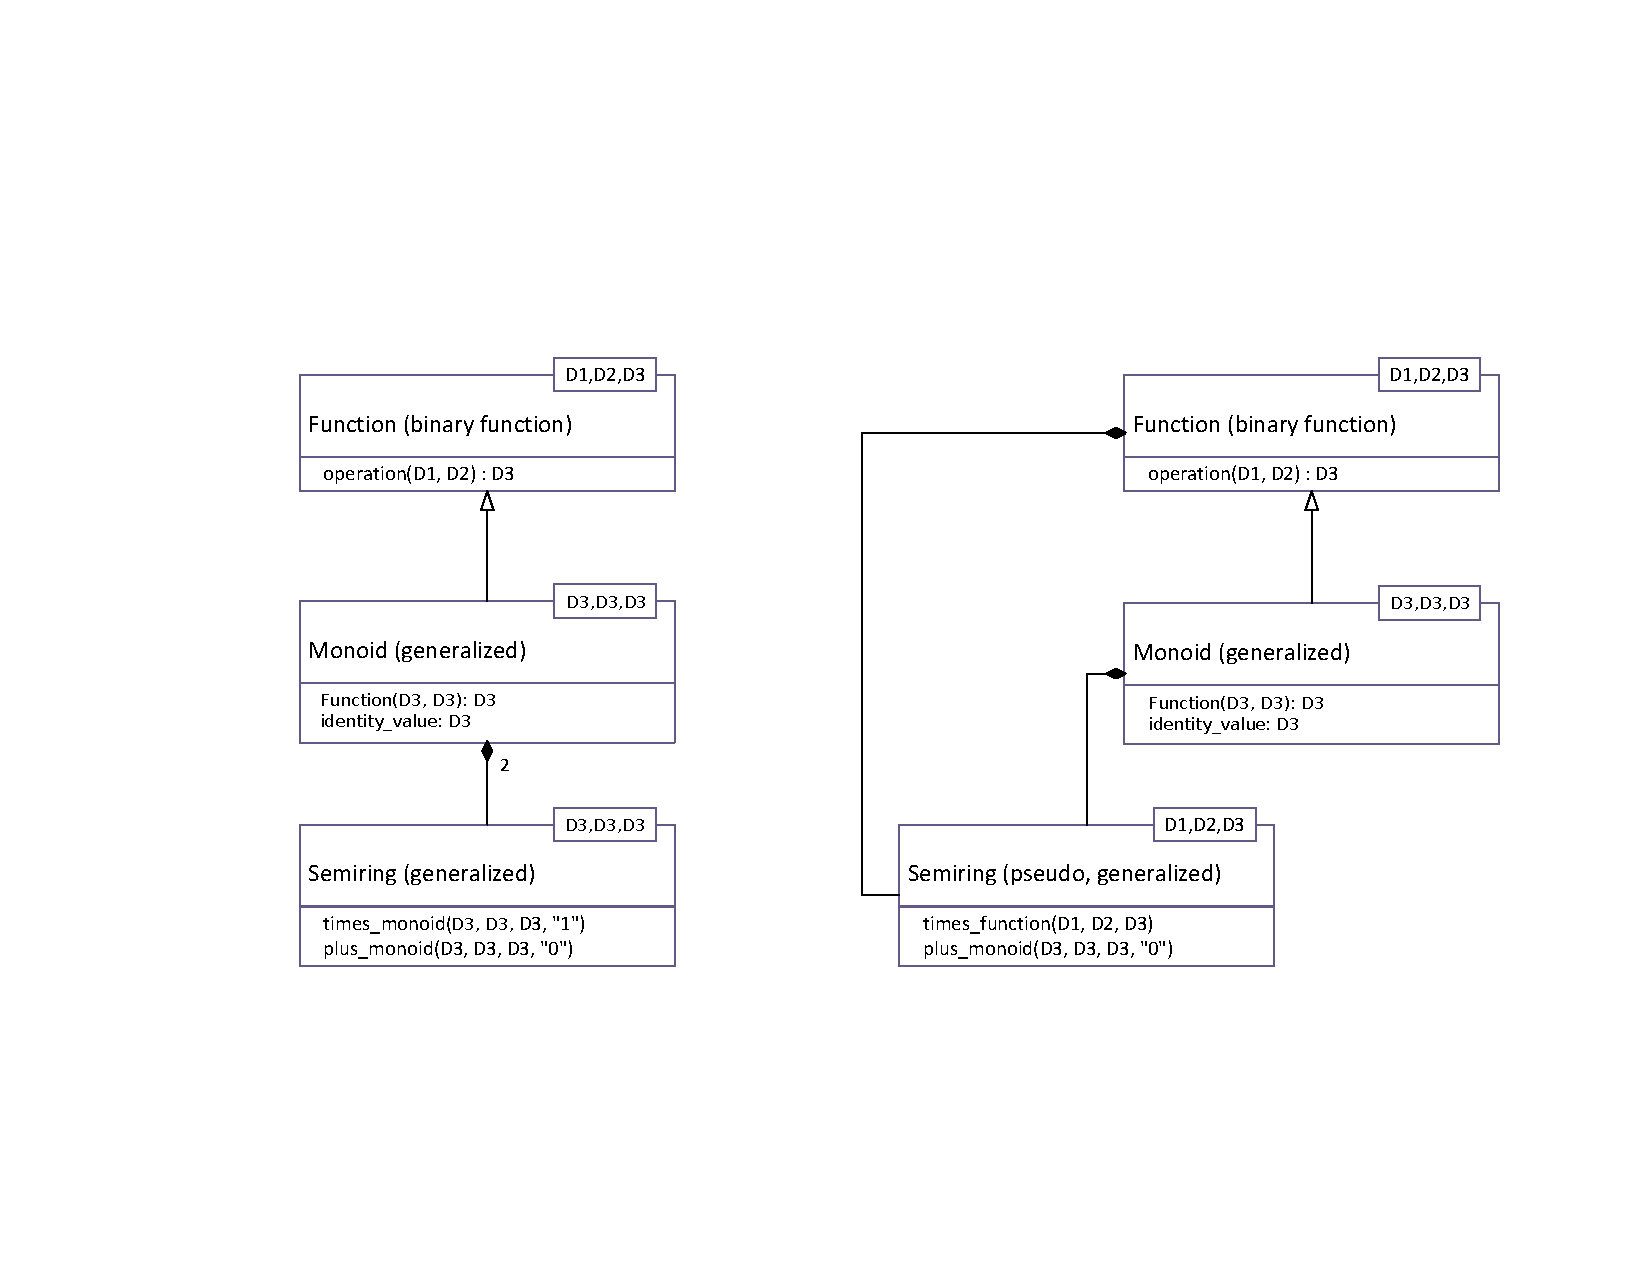
\includegraphics[width=1.0\linewidth,trim=0in 2in 0in 2in]{Algebra_Hierarchy_proposed.pdf}
\end{center}
\caption{Hierarchy of object classes in GraphBLAS algebra.}
\label{Fig:AlgebraHierarchyProposed}
\hrule
\end{figure}

\begin{table}
\hrule
\begin{center}
\caption{Proposed operator input for relevant GraphBLAS operations. The additive operator and multiplicative operator are shown for clarity, and will not be part of the function signature. Every valid input in its most general form is shown in bold. For example, \textbf{Function} is more general than \textbf{Monoid}. \textbf{Monoid} is more general than \textbf{Semiring}.}
\label{Tab:OperatorInputType}
\begin{tabular}{l|l|l|l|l}
Operation	& Operator Input & Additive Operator & Multiplicative Operator & Mapping \\ \hline
\textbf{mXm} & \textbf{Semiring} & \textbf{Monoid} & \textbf{Function} & $D_1 \times D_2 \rightarrow D_3$\\
mXm	 & Semiring & Monoid & Monoid & $D_1 \times D_1 \rightarrow D_1$\\
\textbf{mXv} & \textbf{Semiring} & \textbf{Monoid} & \textbf{Function} & $D_1 \times D_2 \rightarrow D_3$ \\
mXv & Semiring & Monoid & Monoid & $D_1 \times D_1 \rightarrow D_1$ \\
\textbf{ewiseAdd} &  \textbf{Function} & n/a & n/a & $D_1 \times D_2 \rightarrow D_3$ \\
ewiseAdd & Monoid & n/a & n/a & $D_1 \times D_1 \rightarrow D_1$ \\
\textbf{ewiseMult} & \textbf{Function} & n/a & n/a & $D_1 \times D_2 \rightarrow D_3$ \\
ewiseMult & Monoid & n/a & n/a & $D_1 \times D_1 \rightarrow D_1$ \\
\textbf{reduce} & \textbf{Monoid} & n/a & n/a & $D_1 \times D_1 \rightarrow D_1$\\
\end{tabular}
\end{center}
\hrule
\end{table}

\begin{table}
\hrule
\begin{center}
\caption{Proposed function signature for relevant GraphBLAS operations.}
\label{Tab:OperatorInputType}
\begin{tabularx}{\textwidth}{l|X}
Operation	& Function Arguments \\ \hline
mXm	 & GrB\_Vector C, const GrB\_Semiring s, const GrB\_Matrix A, const GrB\_Matrix B[, const GrB\_Matrix M[, const GrB\_Descriptor d]]\\
mXv & GrB\_Vector *u, const GrB\_Semiring s, const GrB\_Matrix A, 
                 const GrB\_vector v[, const GrB\_Vector m[, const GrB\_Descriptor d]] \\
ewiseAdd & GrB\_Vector* w, const GrB\_Monoid s, const GrB\_Vector u,
const GrB\_Vector v[, const GrB\_Vector m[, const GrB\_Descriptor d]] \\
ewiseAdd & GrB\_Vector* w, const GrB\_Function s, const GrB\_Vector u,
const GrB\_Vector v[, const GrB\_Vector m[, const GrB\_Descriptor d]] \\
ewiseMult & GrB\_Vector* w, const GrB\_Monoid s, const GrB\_Vector u,
const GrB\_Vector v[, const GrB\_Vector m[, const GrB\_Descriptor d]] \\
ewiseMult & GrB\_Vector* w, const GrB\_Function s, const GrB\_Vector u,
const GrB\_Vector v[, const GrB\_Vector m[, const GrB\_Descriptor d]] \\
\textbf{reduce} & \\
\end{tabularx}
\end{center}
\hrule
\end{table}
